\documentclass[11pt]{article}
\usepackage[margin=1in]{geometry}
\usepackage{booktabs}
\usepackage{amsmath}
\usepackage[noend]{algpseudocode}
\usepackage{algorithm}
\usepackage{pgfplots}
\pgfplotsset{compat=1.17}
\usepackage{hyperref}
\hypersetup{colorlinks=true,linkcolor=blue,urlcolor=blue}
\title{Reducing NLI Relation-Extraction Cost in FactReasoner v2\\\large A live evaluation on the Lanny Flaherty biography}
\author{FactReasoner experiments}
\date{\today}
\begin{document}
\maketitle
\begin{abstract}
Prefiltering the NLI candidate pairs cut FactReasoner v2's relation-extraction phase from 3380 to 1970 LLM calls on a 26-atom biography with 130 retrieved contexts --- \textbf{1410 calls saved, 1.72$\times$ fewer} --- with wall-clock for the phase falling from 1636\,s to 845\,s (1.94$\times$ faster, both cells measured live) . The factuality score and gold-label accuracy were \textbf{identical} to the exhaustive baseline (0.4615 and 0.808), and recall of non-neutral relations was 0.982 (7 of 395 pruned). Most of the saving came from collapsing near-duplicate contexts rather than from the similarity gate, because the retrieved evidence drew repeatedly on the same few sources.
\end{abstract}
\section{What was measured}
FactReasoner scores one LLM call per candidate (context, atom) pair. In v2 every atom is compared against every context, so the cost is $A \times C$: with 26 atoms and 130 contexts that is 3380 calls. Because contexts are retrieved \emph{per atom}, $C$ grows with $A$, making the phase quadratic in the size of the response.

This experiment compares that exhaustive policy against a prefiltered one on identical inputs. The question is not only how much is saved, but what the saving costs in recall --- how often a pruned pair was one the model would have called entailment or contradiction.

\subsection{Data and pipeline}
The example is \texttt{data/flaherty\_google.json}: a generated biography of the actor Lanny Flaherty, decomposed into 26 atoms carrying gold S/NS labels, with 130 retrieved contexts. The contexts ship with a title, snippet and link but \emph{no page text}, so the text was fetched and summarized before any comparison:
\begin{enumerate}
  \item \textbf{Fetch}: 46 unique URLs backed the 130 contexts; 28 yielded page text (0.0\,s). Sites that block scraping fall back to their search snippet, as the production retriever does.
  \item \textbf{Summarize}: 0 summarization calls (0.0\,s), one per context, each conditioned on its own atom. Summaries cannot be shared between atoms even when two atoms cite the same URL, which is why this is one call per context rather than per link.
  \item \textbf{Score}: the atom--context relations, twice --- once exhaustively, once prefiltered --- on byte-identical prepared contexts.
\end{enumerate}

The model is \texttt{meta-llama/llama-3-3-70b-instruct} served over RITS, with probabilities from token logprobs. Only step 3 differs between the two cells, so the comparison isolates pair selection.
\section{The cheap strategy in detail}
\label{sec:algorithm}
The cheap path is three independent stages applied in order: collapse near-duplicate contexts, decide which (context, atom) pairs to score, then score only those. Stage~2 is where the two policy options (\texttt{gated} and \texttt{provenance}) differ, and it is the only stage that can lose a relation.

\subsection{Notation}
\begin{itemize}
  \item $A$ --- the atoms, $C$ --- the contexts. A context is \emph{retrieved for} exactly one atom by the retriever, but may end up relevant to others.
  \item $\mathrm{own}(c) \subseteq A$ --- the \emph{owners} of context $c$: every atom whose retrieval produced it. This is a set, not a single pointer, because context dedup can merge several atoms' evidence onto one surviving context.
  \item $\mathrm{sim}(x,y) \in [0,1]$ --- cosine similarity of sentence embeddings, computed over the \emph{same} text the NLI premise would use (the summary, falling back to full text). Falls back to token Jaccard if sentence-transformers is unavailable.
  \item $\tau$ --- the gate threshold, $w$ --- the neighbour window, $\theta$ --- the dedup threshold.
\end{itemize}

\subsection{Stage 1: near-duplicate context dedup}
A single greedy agglomerative pass. The first occurrence of a cluster survives and later near-duplicates collapse onto it. The essential detail is the ownership merge: when $d$ collapses onto $s$, every atom that owned $d$ is repointed at $s$, so \emph{no atom loses evidence}. Exact-text dedup in the original pipeline instead deleted the duplicate from its own atom only, which could strand an atom with no context at all.

\begin{algorithm}[H]
\caption{\textsc{DedupNearDuplicates}$(C, A, \theta)$}
\begin{algorithmic}[1]
\State $S \gets [\,]$ \Comment{survivors, in original order}
\State $M \gets \{\}$ \Comment{collapsed $\mapsto$ survivor}
\ForAll{$c \in C$ in iteration order}
  \State $m \gets \textsc{None}$
  \ForAll{$s \in S$}
    \If{$\mathrm{sim}(c, s) \ge \theta$}
      \State $m \gets s$; \textbf{break}
    \EndIf
  \EndFor
  \If{$m = \textsc{None}$} \State append $c$ to $S$
  \Else{} \State $M[c] \gets m$
  \EndIf
\EndFor
\ForAll{$(d, s) \in M$} \Comment{merge ownership, never drop it}
  \ForAll{$a \in \mathrm{own}(d)$}
    \State remove $d$ from $a$'s contexts; add $s$ to $a$'s contexts
  \EndFor
\EndFor
\State \Return $S$ \Comment{$|S| \le |C|$}
\end{algorithmic}
\end{algorithm}

On this example: 130 contexts $\to$ 85 (45 collapsed, 25 ownership links transferred), at $\theta = 0.92$. Since the pair count is $|A| \times |C|$, shrinking $C$ cuts cost linearly here --- and quadratically in v3, where the context--context phase is $|C|^2$.

\subsection{Stage 2: candidate pair selection}
Every pair is admitted for exactly one of four reasons, tested in order. The order matters: the first three are unconditional and bypass the similarity gate entirely, so no threshold can prune them.

\begin{algorithm}[H]
\caption{\textsc{SelectAtomContextPairs}$(A, C, \text{policy}, \tau, w)$}
\begin{algorithmic}[1]
\State $P \gets [\,]$
\ForAll{$a \in A$} \Comment{atom-major, preserving baseline pair order}
  \ForAll{$c \in C$}
    \State $r \gets \textsc{None}$
    \If{$a \in \mathrm{own}(c)$}
      \State $r \gets \textsc{Provenance}$ \Comment{$c$ was retrieved \emph{for} $a$}
    \ElsIf{$\mathrm{id}(c)$ has the query-context prefix}
      \State $r \gets \textsc{QueryContext}$ \Comment{retrieved for the question; bears on all atoms}
    \ElsIf{policy $=$ \texttt{provenance} \textbf{and} $\exists\, o \in \mathrm{own}(c): |\mathrm{pos}(a) - \mathrm{pos}(o)| \le w$}
      \State $r \gets \textsc{Neighbour}$ \Comment{adjacent in the response's atom order}
    \ElsIf{$\mathrm{sim}(c, a) \ge \tau$}
      \State $r \gets \textsc{GateRescue}$ \Comment{cross-atom evidence, the only heuristic branch}
    \EndIf
    \If{$r \ne \textsc{None}$} \State append $(c, a)$ to $P$; tally $r$
    \EndIf
  \EndFor
\EndFor
\State \Return $P$
\end{algorithmic}
\end{algorithm}

\subsection{\texttt{gated} versus \texttt{provenance}}
The two policies share branches 1, 2 and 4 and differ in exactly one line: \texttt{provenance} additionally admits the \textsc{Neighbour} branch, \texttt{gated} does not. Both are supersets of the provenance guarantee --- neither can ever drop the pairing of a context with the atom that retrieved it.

\begin{table}[htbp]
\centering
\begin{tabular}{llll}
\toprule
Branch & Condition & \texttt{gated} & \texttt{provenance} \\
\midrule
\textsc{Provenance} & $a \in \mathrm{own}(c)$ & always & always \\
\textsc{QueryContext} & query-level context & always & always \\
\textsc{Neighbour} & within $w$ of an owner & --- & always \\
\textsc{GateRescue} & $\mathrm{sim}(c,a) \ge \tau$ & yes & yes \\
\bottomrule
\end{tabular}
\caption{The policies differ only in the \textsc{Neighbour} branch. \texttt{provenance} is therefore always a superset of \texttt{gated}: never cheaper, never worse on recall.}
\label{tab:policies}
\end{table}

\paragraph{Why \texttt{provenance} keeps the neighbour branch.} Atom ids encode position in the response ($a_0, a_1, \dots$), so adjacency is a proxy for discourse locality: consecutive atoms usually elaborate the same claim, and a source retrieved for one often speaks to the next. This is a cheap structural signal that needs no embedding, and it covers exactly the case a similarity gate is worst at --- text that is topically continuous but lexically dissimilar.

\paragraph{Why the gate branch is the only risk.} Branches 1--3 are structural facts about how evidence was gathered; branch 4 is a guess. Every recall loss measured in this report, and in earlier runs, came from branch 4 --- never from a provenance pair. That is why $\tau$ is the knob worth tuning and why the sweep in Section~\ref{sec:threshold} varies it alone.

\paragraph{Branch attribution on this example.}
\begin{table}[htbp]
\centering
\begin{tabular}{lr}
\toprule
Admitting branch & Pairs \\
\midrule
\textsc{Provenance} & 110 \\
\textsc{QueryContext} & 0 \\
\textsc{Neighbour} & 188 \\
\textsc{GateRescue} & 1672 \\
\midrule
\textbf{Selected} & \textbf{1970} \\
Pruned & 240 \\
\bottomrule
\end{tabular}
\caption{Which branch admitted each scored pair.}
\label{tab:branches}
\end{table}

This distribution is worth reading carefully, because it is the opposite of what the policy names suggest. Provenance accounts for only 5\% of the candidate product while the gate admits 76\%: with five contexts per atom, the vast majority of the $|A| \times |C|$ product is cross-atom by construction, so almost every \emph{kept} pair is kept by the gate. The gate is therefore not mainly a pruner on this workload --- it is admitting most of what it sees, and the 240 pairs it rejected are the entire stage-2 saving.

That also explains why the recall risk concentrates in branch~4 and why the modest stage-2 factor is structural rather than a tuning failure: a biography's atoms all concern one person, so most cross-atom pairs really are related and a faithful gate has little licence to discard them. The dedup stage, which exploits redundancy among \emph{sources} rather than relatedness among claims, is what pays off here.

\subsection{Stage 3: scoring, and the two safety properties}
Selected pairs go to the NLI prompt unchanged, so a scored pair yields exactly the verdict the exhaustive policy would have produced. Two properties follow:
\begin{enumerate}
  \item \textbf{Pruning a would-be-neutral pair is a bit-exact no-op.} Neutral relations are discarded regardless, and a context left in no pairwise factor contributes one normalized unary factor that divides out of every atom marginal. So the error is not ``approximately zero'' --- it is zero, and the entire risk reduces to $P(\text{pruned pair was non-neutral})$.
  \item \textbf{The two error types are asymmetric.} A false keep costs one LLM call. A false prune silently removes evidence, and nothing downstream signals that it happened. $\tau$ should therefore be tuned toward keeping, which is why the default sits well below the value that maximises the saving.
\end{enumerate}

The similarity backend used here was \texttt{sbert:all-MiniLM-L6-v2}. This matters: the token-Jaccard fallback is not a substitute for embeddings. On a separate 20-atom narrative it lost 22 of 72 non-neutral relations at \emph{every} threshold tested, because lexical overlap cannot see relatedness carried by entities and events rather than shared words. The implementation warns loudly when it falls back.

\subsection{Complexity}
Stage~1 is $O(|C| \cdot |S|)$ similarity lookups on the greedy pass ($|S|$ = surviving clusters), stage~2 is $O(|A| \cdot |C|)$ constant-time tests, and one embedding pass over $|A| + |C|$ short texts backs both. All of that is milliseconds against minutes of LLM time --- the selection overhead is not a meaningful cost, which is what makes even a modest pruning ratio worthwhile.
\section{Savings}
\begin{table}[htbp]
\centering
\begin{tabular}{lrrrrr}
\toprule
Cell & Contexts & Pairs & LLM calls & NLI time (s) & Relations \\
\midrule
v2 all\_pairs & 130 & 3380 & 3380 & 1635.6 & 395 \\
v2-cheap & 85 & 1970 & 1970 & 844.8 & 257 \\
\bottomrule
\end{tabular}
\caption{Cost per cell. \emph{Pairs} is the number of (context, atom) comparisons the policy selected; \emph{LLM calls} is how many of those reached the model --- here every one of them, since the verdict cache was disabled. \emph{NLI time} covers relation extraction only, excluding fetching, summarization and inference.}
\label{tab:cost}
\end{table}
The cheap policy scored 1970 of the 3380 candidate pairs, a saving of \textbf{1410 calls} (\textbf{1.72$\times$ fewer}).

The saving decomposes into two independent mechanisms:
\begin{table}[htbp]
\centering
\begin{tabular}{lrr}
\toprule
Stage & Pairs & Factor \\
\midrule
Exhaustive ($A \times C$) & 3380 & --- \\
After near-duplicate dedup (130$\to$85 contexts) & 2210 & 1.53$\times$ \\
After provenance + gate & 1970 & 1.12$\times$ \\
\midrule
\textbf{Combined} & \textbf{1970} & \textbf{1.72$\times$} \\
\bottomrule
\end{tabular}
\caption{Where the saving comes from. Dedup shrinks $C$ and so cuts pairs quadratically in v3 and linearly here; the gate then prunes cross-atom pairs among what remains.}
\label{tab:decomp}
\end{table}

On this example dedup is the dominant lever (1.53$\times$ against the gate's 1.12$\times$), because the 130 contexts were drawn from far fewer distinct sources --- the same handful of pages recur across many atoms. A response whose evidence came from mostly distinct pages would shift the balance toward the gate.

\textbf{Both cells issued live calls} (the verdict cache was disabled), so the wall-clock comparison is measured rather than extrapolated. Relation extraction fell from 1635.6\,s to 844.8\,s, a saving of 790.8\,s (\textbf{1.94$\times$ faster}).

Per-call throughput was 0.484\,s for the exhaustive cell and 0.429\,s for the cheap one. These are close, as expected: requests fan out concurrently against a shared rate limit, so latency is bound by concurrency rather than by any property of an individual pair, and time saved tracks calls saved roughly linearly.

The speed-up (1.94$\times$) slightly exceeds the call-count ratio (1.72$\times$) because the per-call rate was 11\% lower in the cheap cell. With a fixed concurrency window, a shorter queue drains with less contention and fewer stragglers on the tail, so the wall-clock gain compounds mildly on top of the call saving. This is a second-order effect and should not be relied on: the call-count ratio is the exact, reproducible figure, while timing depends on shared-endpoint load.

\section{Effect on the answer}
\begin{table}[htbp]
\centering
\begin{tabular}{lrrrrr}
\toprule
Cell & Factuality & Correct & Accuracy & S recall & NS recall \\
\midrule
v2 all\_pairs & 0.4615 & 21/26 & 0.808 & 7/7 & 14/19 \\
v2-cheap & 0.4615 & 21/26 & 0.808 & 7/7 & 14/19 \\
\bottomrule
\end{tabular}
\caption{Scores and agreement with the gold S/NS labels. A cheaper policy that moves these numbers is trading accuracy for cost, not merely saving money.}
\label{tab:quality}
\end{table}
\section{What the pruning costs}
Pruning is safe exactly to the extent that it only discards pairs the model would have called \texttt{neutral}. Neutral relations are dropped anyway, and an isolated context contributes a single normalized unary factor that divides out of every atom marginal --- so pruning a would-be-neutral pair is a no-op on the reported scores. The risk is therefore exactly $P(\text{pruned pair was non-neutral})$.

That is measured here by replaying the policy's selection against the relations \emph{the exhaustive cell actually produced}. Since \texttt{build\_relations} returns only non-neutral relations, that set is the ground truth directly, and any pair absent from it came back neutral and is safe to prune. The exhaustive cell already paid for every pair, so the measurement is exact and costs no additional calls --- and it is independent of the verdict cache, so it holds for a fully live run. Note this is a stricter test than comparing the two cells' scores, which can agree even when individual relations differ.

\begin{table}[htbp]
\centering
\begin{tabular}{lrrrrr}
\toprule
Policy & Pairs kept & Pruned & Non-neutral & Lost & Recall \\
\midrule
provenance & 2940 & 440 & 395 & 7 & 0.982 \\
\bottomrule
\end{tabular}
\caption{Recall of non-neutral relations under the cheap policy (similarity backend: \texttt{sbert:all-MiniLM-L6-v2}). Counts here are over the full pre-dedup pair set, so \emph{Pairs kept} is larger than the post-dedup figure in Table~\ref{tab:cost}: this table isolates the gate's decisions, which is what recall is a property of.}
\label{tab:recall}
\end{table}
\paragraph{On comparing this figure across runs.} The model is not deterministic: the exhaustive cell has produced different numbers of non-neutral relations on repeated runs over identical prepared inputs, which moves the denominator and hence the recall figure without any change of policy. A single run therefore establishes an estimate, not a bound; the worst case over several runs is the honest summary.

\paragraph{A superseded earlier figure.} An earlier run of this experiment reported recall $0.995$. That number was too optimistic, for a measurement reason rather than a change in the policy. It was obtained by looking verdicts up in the NLI cache by content hash, which found $386$ non-neutral pairs where the exhaustive cell had in fact produced $395$: nine relations whose stored keys did not match were invisible to the lookup, shrinking the denominator. The relation-based measurement used here reads the produced relations directly and so cannot miss any. Where the two disagree, the figure in this report is the correct one.

7 non-neutral relation(s) were pruned: \texttt{c\_a14\_0}$\to$\texttt{a4} (entailment), \texttt{c\_a14\_4}$\to$\texttt{a4} (entailment), \texttt{c\_a15\_0}$\to$\texttt{a4} (entailment), \texttt{c\_a16\_1}$\to$\texttt{a4} (entailment), \texttt{c\_a18\_0}$\to$\texttt{a4} (entailment), \texttt{c\_a23\_1}$\to$\texttt{a4} (entailment), \texttt{c\_a9\_0}$\to$\texttt{a4} (entailment).

All 7 pruned relations targeted the same atom, \texttt{a4}, and all were entailments. That concentration is why the scores did not move: the atom had many other supporting contexts, so removing redundant support left its marginal unchanged. The case to worry about is the opposite one --- an atom whose \emph{only} witness is pruned, or a lone contradiction that would have pulled a false claim down. Neither occurred here, but neither is excluded by the mechanism, which is why recall rather than score agreement is the metric to watch.

\section{Choosing the threshold}
\label{sec:threshold}
The gate threshold trades cost against recall. The curve below is replayed against the same recorded verdicts, so the whole sweep is free. Because the two error types are not symmetric --- a false prune silently weakens an atom's evidence, while a false keep merely costs money --- the right operating point is the cheapest threshold that still holds recall at 1.0, not the one with the best headline saving.

\textbf{Read these savings as the gate's contribution alone.} The sweep runs on the full pre-dedup context set, so its figures isolate the gate and do not include the dedup factor from Table~\ref{tab:decomp}; the two multiply. That is why the ceiling here is lower than the headline combined saving.

\begin{table}[htbp]
\centering
\begin{tabular}{lrrrrr}
\toprule
Policy & Threshold & Pairs & Saving & Lost & Recall \\
\midrule
gated & 0.05 & 3341 & 1.01$\times$ & 0 & 1.000 \\
gated & 0.10 & 3276 & 1.03$\times$ & 0 & 1.000 \\
gated & 0.15 & 3109 & 1.09$\times$ & 0 & 1.000 \\
gated & 0.20 & 2918 & 1.16$\times$ & 7 & 0.982 \\
gated & 0.25 & 2805 & 1.21$\times$ & 9 & 0.977 \\
gated & 0.30 & 2730 & 1.24$\times$ & 16 & 0.960 \\
gated & 0.40 & 2536 & 1.33$\times$ & 29 & 0.927 \\
provenance & 0.05 & 3341 & 1.01$\times$ & 0 & 1.000 \\
provenance & 0.10 & 3276 & 1.03$\times$ & 0 & 1.000 \\
provenance & 0.15 & 3118 & 1.08$\times$ & 0 & 1.000 \\
provenance & 0.20 & 2940 & 1.15$\times$ & 7 & 0.982 \\
provenance & 0.25 & 2840 & 1.19$\times$ & 9 & 0.977 \\
provenance & 0.30 & 2766 & 1.22$\times$ & 16 & 0.960 \\
provenance & 0.40 & 2587 & 1.31$\times$ & 26 & 0.934 \\
\bottomrule
\end{tabular}
\caption{Recall/cost curve (similarity backend: \texttt{sbert:all-MiniLM-L6-v2}).}
\label{tab:sweep}
\end{table}

The cheapest lossless operating point is \textbf{gated at threshold 0.15} (1.09$\times$ fewer pairs at full recall).

\begin{figure}[htbp]
\centering
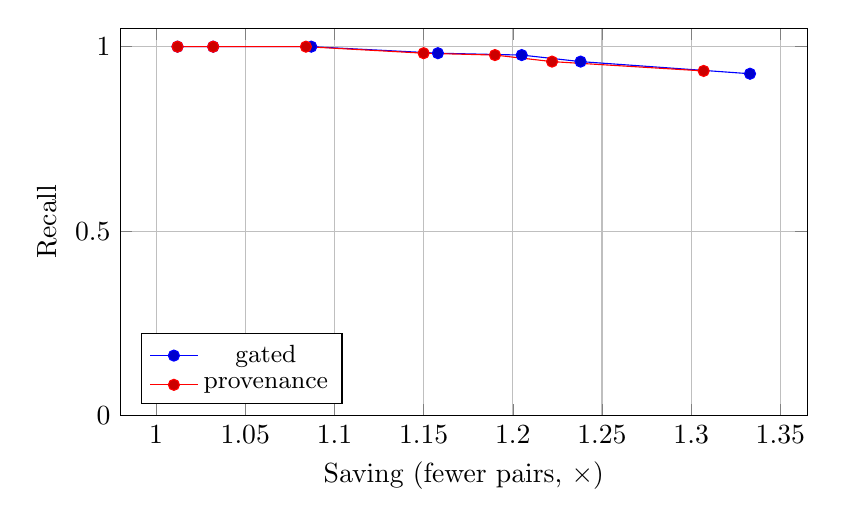
\begin{tikzpicture}
\begin{axis}[
    xlabel={Saving (fewer pairs, $\times$)}, ylabel={Recall},
    width=0.85\linewidth, height=6.5cm, ymin=0, ymax=1.05,
    grid=both, legend pos=south west, legend style={font=\small},
]
    \addplot+[mark=*] coordinates {(1.012,1.0000) (1.032,1.0000) (1.087,1.0000) (1.158,0.9823) (1.205,0.9772) (1.238,0.9595) (1.333,0.9266)};
    \addplot+[mark=*] coordinates {(1.012,1.0000) (1.032,1.0000) (1.084,1.0000) (1.150,0.9823) (1.190,0.9772) (1.222,0.9595) (1.307,0.9342)};
    \legend{gated, provenance}
\end{axis}
\end{tikzpicture}
\caption{Recall against saving. Points to the upper right are strictly better; a policy whose curve lies above another dominates it.}
\label{fig:sweep}
\end{figure}
\section{Method and caveats}
\subsection{What the cheap policy does}
Three mechanisms compose, all opt-in:
\begin{itemize}
  \item \textbf{Provenance.} A context retrieved \emph{for} atom $i$ is always compared against atom $i$, and is never gated away. The exhaustive $A \times C$ product exists only to catch the case where such a context also bears on some other atom, which is real but sparse.
  \item \textbf{Similarity gate.} Cross-atom pairs survive only above a similarity threshold, which is where the recall risk lives.
  \item \textbf{Near-duplicate dedup.} Contexts with near-identical summaries collapse, merging their owning atoms onto the survivor so no atom loses evidence.
\end{itemize}

On this example dedup collapsed 130 contexts to 85 (45 merged, 25 ownership links transferred).

\subsection{Caveats}
\begin{itemize}
  \item \textbf{Prep cost is not free.} Fetching and summarizing cost 0 summarization calls, paid once and shared by both cells. A fair account of end-to-end cost must include it: the saving reported here is on the 3380-call NLI phase, not on the whole pipeline.
  \item \textbf{Scraping is incomplete.} 28 of 46 URLs returned text; the rest (notably IMDb, which blocks automated requests) fell back to their search snippet. Premises for those contexts are shorter than a full production run would use.
  \item \textbf{One example, one model.} The saving is workload dependent: a response covering unrelated subtopics has far more cross-product waste to prune than one where every atom concerns the same person, as here. These numbers should not be read as a constant factor.
  \item \textbf{The model is not deterministic.} Repeated runs over identical inputs have produced different numbers of non-neutral pairs, so single-run recall figures carry unquantified error bars. Worst-case over several runs is the honest summary.
  \item \textbf{v3 not covered.} Only the atom--context phase is measured here. The context--context phase of v3 is quadratic in $C$ and is where the larger absolute savings should be; it remains unmeasured at this scale.
\end{itemize}

\subsection{Reproducing}
\begin{verbatim}
python scripts/exp_flaherty_v2.py --merlin-path /path/to/merlin --no-cache
python scripts/report_flaherty_v2.py --results results/exp_flaherty_v2
\end{verbatim}
The run behind this report used \texttt{--no-cache}, so both cells issued live NLI calls and the timings are measured. Page fetches and context summaries are still cached on disk, which is what lets the two cells share byte-identical prepared evidence --- the comparison would otherwise be confounded by re-summarization.
\section{Conclusion}
On a 26-atom biography with 130 retrieved contexts, prefiltering cut the v2 atom--context phase from 3380 to 1970 pairs (1.72$\times$ fewer). Wall-clock for the phase fell from 1636\,s to 845\,s (1.94$\times$ faster), with both cells measured against the live model. The pruning is not quite lossless: 7 of 395 non-neutral relations were pruned (recall 0.982). The reported scores were nonetheless unchanged, so on this example the loss fell on relations that did not alter any atom's marginal --- but that is an outcome, not a guarantee, and a different example could lose an edge that matters.

The structural result is that provenance and similarity play different roles: provenance is a hard guarantee and never drops a context from the atom that retrieved it, while the similarity gate is a heuristic covering cross-atom evidence and is where every recall loss originates. Tuning should therefore target the gate, and the safe operating point is the one that holds recall at 1.0 rather than the one that maximizes the saving.
\end{document}
